% ---------------------------------------------------------------------
\Needspace{8\baselineskip}\subsection{Le dashboard}

Le dashboard existe déjà pour afficher les mesures. Je le complète pour qu'il devienne le poste de commande du pilotage : la tour n'a ni clavier ni grand écran, et je veux pouvoir tout régler depuis un téléphone. Je veux aussi comprendre à tout moment pourquoi la tour a agi, d'où l'importance des alertes et du journal.

Le dashboard est une page web servie par le Raspberry, à l'adresse \texttt{http://<ip-du-raspberry>:5000}. On l'ouvre depuis n'importe quel téléphone ou ordinateur du même réseau Wi-Fi ; elle se met à jour toutes les 10 secondes. Les captures ci-dessous sont faites avec un Arduino simulé (partie 8.9) ; l'accès depuis Internet et sa page de connexion sont présentés dans la partie 8.6. Cette sous-partie présente le dashboard onglet par onglet : d'abord les mesures, puis la tour en 3D et la commande manuelle des pompes, et enfin les réglages du pilotage et l'étalonnage des sondes.

\subsubsection*{Les mesures}

Sur l'onglet Mesures, je veux qu'on voie en un coup d'œil si tout va bien. Chaque mesure est comparée à la cible du légume, et les alertes du Raspberry s'ajoutent au bandeau du haut. J'ajoute aussi la pression, et j'affiche la lumière en pourcentage : le capteur du Sensor Kit n'est pas étalonné, et afficher des lux serait trompeur.

\begin{figure}[H]
\centering
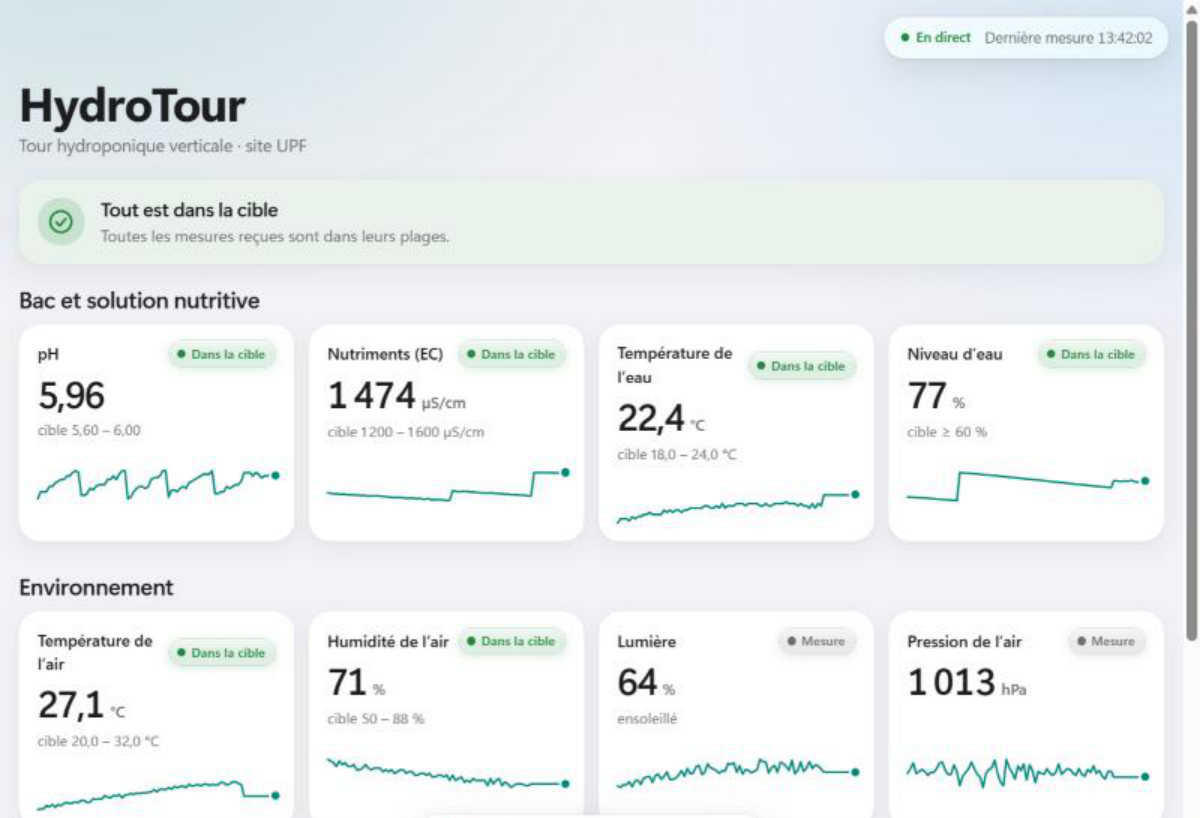
\includegraphics[width=\textwidth]{img/inf/d_mesures.png}
\caption{Onglet Mesures : chaque tuile indique la valeur, la cible du légume et la courbe des 6 dernières heures. Le bandeau du haut résume l'état et affiche les alertes du pilote.}
\end{figure}

\subsubsection*{La tour et les pompes}

La commande manuelle reste indispensable pour les essais et l'entretien. Je décide qu'un appui manuel sur la circulation mette l'automatique en pause : sinon, le Raspberry rallumerait la pompe dix secondes plus tard, et on ne comprendrait pas pourquoi. Je retire la pompe d'eau claire de l'affichage sur la vraie tour, puisqu'elle n'existe que dans la démonstration.

La figure suivante montre l'onglet Installation du dashboard.

\begin{figure}[H]
\centering
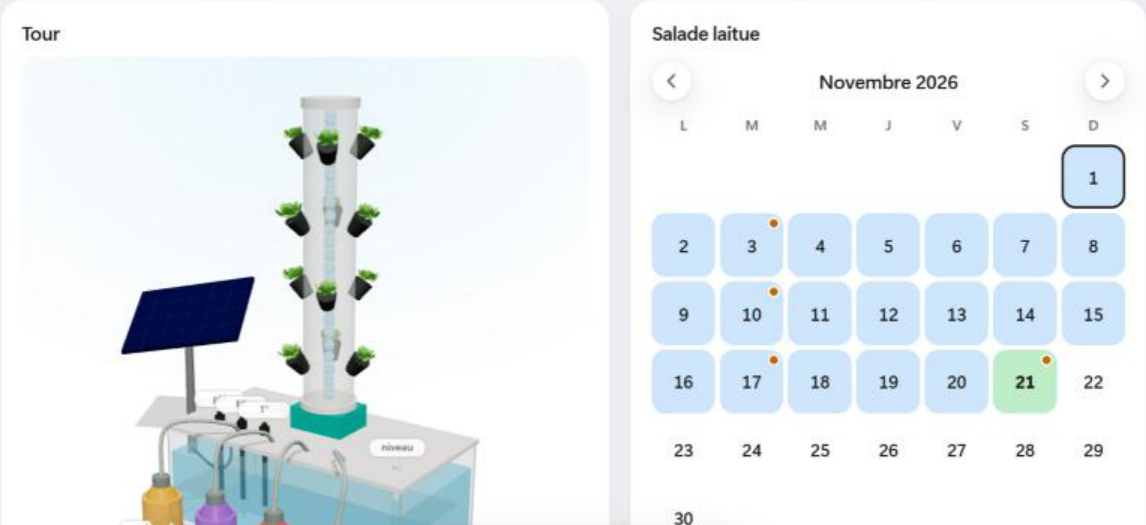
\includegraphics[width=\textwidth]{img/inf/d_tour.png}
\caption{Onglet Installation : la tour en 3D suit le stade du légume, et le calendrier rappelle les contrôles à faire.}
\end{figure}

La carte des pompes montre l'état de chacune. Le bouton Arrêter / Démarrer commande la circulation à la main : le pilotage automatique se met alors en pause, jusqu'à ce qu'on le réactive dans les paramètres. Les boutons Doser 3 s lancent une dose manuelle. Le stock d'engrais restant est rappelé sous chaque doseuse.

La figure suivante montre la carte des pompes.

\begin{figure}[H]
\centering
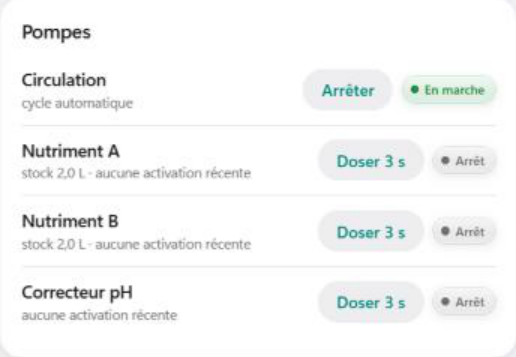
\includegraphics[width=0.6\textwidth]{img/inf/d_pompes.png}
\caption{Carte des pompes.}
\end{figure}

\subsubsection*{Les paramètres}

Les seuils de batterie conseillés ne conviennent pas forcément à toutes les situations : je choisis donc de les laisser réglables, tout en affichant un conseil quand on descend sous \qty{30}{\percent} ou \qty{35}{\percent}. Le serveur vérifie aussi les valeurs reçues, pour qu'une erreur de saisie ne puisse pas bloquer la pompe.

La figure suivante montre les réglages du pilotage et l'étalonnage.

\begin{figure}[H]
\centering
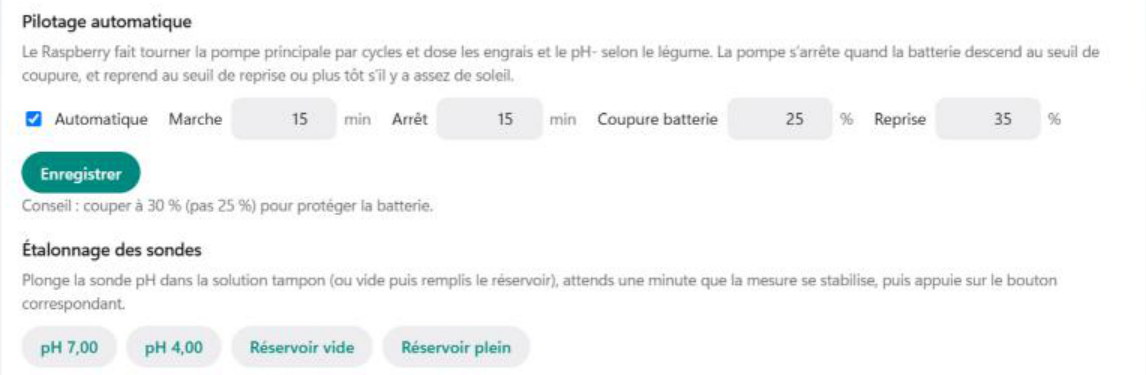
\includegraphics[width=\textwidth]{img/inf/d_param.png}
\caption{Réglages du pilotage et étalonnage. Avec une coupure à 25 \%, le dashboard conseille de couper à 30 \%.}
\end{figure}

Le bloc Pilotage automatique règle le cycle de la pompe et les seuils de la batterie ; le serveur refuse une reprise trop proche de la coupure. Le bloc Étalonnage des sondes enregistre la mesure du moment comme référence : pH 7 et pH 4 dans les solutions tampon, réservoir vide et plein. Le choix du légume et de sa date de plantation est envoyé au Raspberry, qui adapte aussitôt ses cibles. Enfin, le bloc Accès, en haut des paramètres, permet de changer l'identifiant et le mot de passe du site et de se déconnecter (partie 8.6).

% ---------------------------------------------------------------------
\Needspace{8\baselineskip}\subsection{Accès à distance et sécurité}

Jusqu'ici, le dashboard ne s'ouvre que depuis le Wi-Fi de la maison. Or la tour doit tourner seule pendant des jours : je veux pouvoir vérifier le pH ou la batterie depuis l'université, et réagir à une alarme sans être sur place. Mettre la tour sur Internet pose une nouvelle question : comment empêcher n'importe qui de commander les pompes ? Je cherche une solution gratuite, simple à installer sur le Raspberry, et qui ne m'oblige pas à toucher aux réglages de la box.

Cette sous-partie explique le choix de Tailscale\ix{20} Funnel\ix{20} pour rendre la tour joignable depuis Internet, puis la première version de la protection, trop compliquée, et la solution simple que je retiens. Elle présente ensuite la page de connexion, avec son identifiant, son mot de passe et son captcha, et se termine par les deux portes d'entrée du serveur et ce qui est protégé.

\subsubsection*{Rendre la tour joignable depuis Internet}

Le Raspberry est branché derrière la box de la maison : depuis Internet, on ne peut pas l'atteindre directement. Je compare trois solutions :

\begin{table}[H]
\centering
\small
\begin{tabularx}{\textwidth}{|l|Y|Y|}
\hline
\textbf{Solution} & \textbf{Avantages} & \textbf{Inconvénients} \\
\hline
Ouvrir un port de la box & aucun service extérieur & le Raspberry est exposé directement ; dépend de la box et de l'opérateur ; certificat https à gérer soi-même \\
\hline
Cloudflare Tunnel & gratuit, https, rien à ouvrir sur la box & demande un nom de domaine payant (environ 10 euros par an) pour une adresse fixe \\
\hline
Tailscale\ix{20} Funnel\ix{20} (retenu) & gratuit, https, adresse fixe en \texttt{.ts.net}, rien à ouvrir sur la box & dépend du service Tailscale\ix{20} \\
\hline
\end{tabularx}
\caption{Comparaison des trois solutions d'accès depuis Internet.}
\end{table}

Je retiens Tailscale\ix{20} Funnel\ix{20}. Un petit programme installé sur le Raspberry ouvre lui-même une connexion vers Tailscale\ix{20} ; les visiteurs passent par Tailscale\ix{20}, qui leur fournit le https et transmet leurs demandes au Raspberry. La box ne voit qu'une connexion sortante, comme pour n'importe quel site visité. L'adresse publique ne change jamais, et une seule commande suffit pour publier le serveur : \texttt{sudo tailscale funnel --bg 5001}.

\subsubsection*{Une première version trop compliquée}

Je conçois d'abord une gestion complète des comptes : un compte administrateur qui crée des comptes lecteurs, chacun avec son identifiant, son mot de passe et son adresse mail ; des mots de passe provisoires à changer à la première connexion ; et un lien de réinitialisation envoyé par mail, valable 15 minutes. Avant de l'écrire, j'évalue ce qu'elle demande : une base des comptes, une page d'administration, l'envoi de mails par le Gmail du projet\ldots{} J'en écris et j'en teste une première version.

En la reprenant, je me rends compte qu'elle est disproportionnée : la tour n'a que quelques utilisateurs, qui se connaissent tous. J'annule donc tout au profit d'une solution simple : un seul identifiant et un seul mot de passe, partagés. Quiconque les connaît a tous les droits. Le prix de cette simplicité est connu : on ne sait pas qui a fait quoi, et pour retirer l'accès à quelqu'un, il faut changer le mot de passe de tout le monde. Pour ce projet, ce compromis me paraît raisonnable.

\subsubsection*{La page de connexion}

Toute visite commence par une page de connexion, aussi bien depuis Internet que depuis le Wi-Fi de la maison : un invité branché sur le Wi-Fi ne doit pas pouvoir commander les pompes. La page demande trois choses : l'identifiant, le mot de passe et un captcha.

La figure suivante montre la page de connexion, avec son captcha.

\begin{figure}[H]
\centering
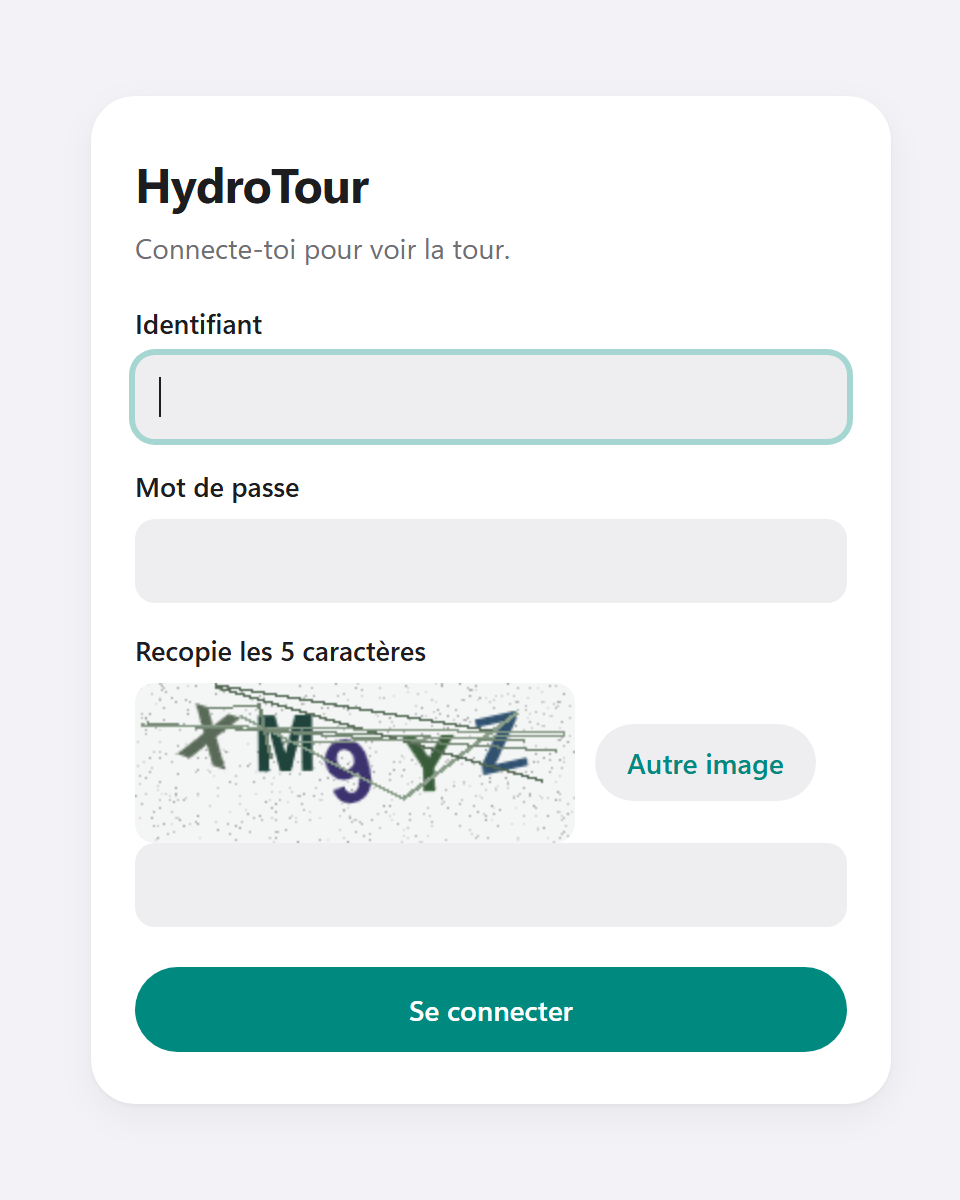
\includegraphics[width=0.5\textwidth]{img/inf/d_login.png}
\caption{La page de connexion, avec son captcha.}
\end{figure}

Le captcha est fait maison : le Raspberry dessine une image de cinq caractères penchés, de couleurs différentes, barrés de traits, avec la bibliothèque Pillow déjà utilisée pour l'écran. Je retire les caractères qui se confondent (0 et O, 1, I et L). Chaque image ne sert qu'une seule fois et expire au bout de 10 minutes : un robot ne peut pas réutiliser une réponse trouvée une fois. Le nombre d'essais n'est pas limité : c'est un choix volontaire, le captcha suffisant à ralentir un robot qui essaierait des mots de passe au hasard.

\begin{itemize}
\item \textbf{Mot de passe protégé} : il n'est jamais enregistré en clair, seulement son empreinte (hachage scrypt) ; même en lisant la base de données, on ne peut pas le retrouver.
\item \textbf{Premier lancement} : le serveur crée l'identifiant \texttt{hydrotour} avec un mot de passe provisoire, affiché sur le Raspberry et écrit dans un fichier qui s'efface dès qu'on le change.
\item \textbf{Changement} : dans Paramètres $>$ Accès, en redonnant l'ancien mot de passe. Tous les autres appareils sont alors déconnectés.
\item \textbf{Session} : on reste connecté 30 jours, ou jusqu'au bouton « Se déconnecter ».
\item \textbf{Oubli} : sur le Raspberry, la commande \texttt{python acces.py secours} crée un nouveau mot de passe provisoire.
\end{itemize}

\subsubsection*{Deux portes d'entrée}

En préparant la protection, je rencontre une difficulté : Tailscale\ix{20} transmet les visites d'Internet au Raspberry depuis le Raspberry lui-même (adresse 127.0.0.1). Pour le serveur, un visiteur venu d'Internet ressemble donc à un appareil de la maison. Or certaines demandes ne doivent venir que de la maison, comme \texttt{/api/data}, par laquelle un ancien Arduino Wi-Fi envoie ses mesures sans mot de passe. Je résous le problème en donnant au serveur deux portes :

Le schéma suivant montre les deux portes d'entrée du serveur et la règle commune.

\begin{figure}[H]
\centering
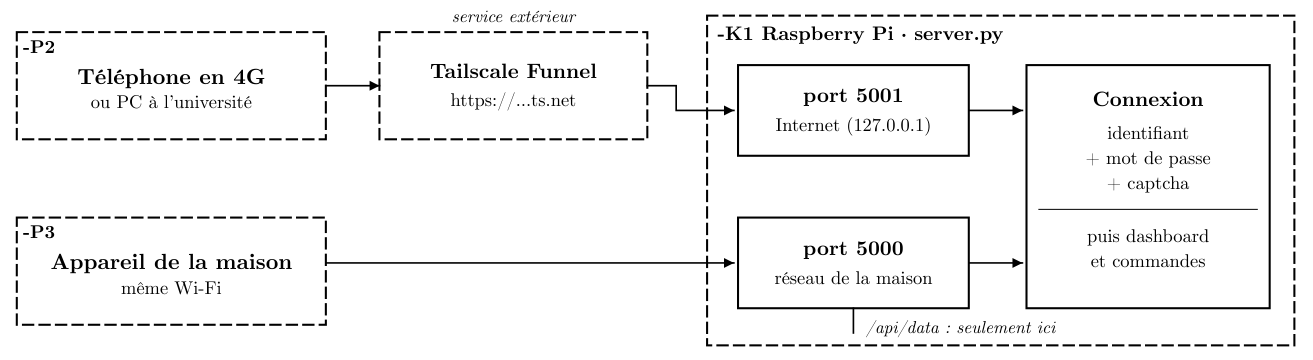
\includegraphics[width=\textwidth]{img/inf/f_portes.png}
\caption{Deux portes d'entrée, une seule règle : il faut se connecter. Seule la porte de la maison accepte aussi les mesures envoyées sans mot de passe.}
\end{figure}

La porte 5001 n'écoute que sur le Raspberry lui-même : seul Tailscale\ix{20} peut l'utiliser, et tout ce qui y arrive est traité comme venant d'Internet. La porte 5000 sert le réseau de la maison. Les deux demandent la connexion ; seule la porte 5000 accepte en plus \texttt{/api/data}, et seulement depuis une adresse locale. Je retire aussi une autorisation qui laisse n'importe quel site lire les mesures (en-tête CORS « $*$ »), et j'interdis l'affichage du dashboard à l'intérieur d'un autre site.

\begin{aretenir}
Sans connexion, seules la page de connexion et l'image du captcha répondent ; toute autre demande est renvoyée vers la connexion. Je vérifie chaque cas par des essais automatiques (23 cas : mauvais captcha, captcha réutilisé, mauvais mot de passe, déconnexion des autres appareils\ldots), puis depuis l'adresse publique : \texttt{/api/data} y est bien refusée.
\end{aretenir}

% ---------------------------------------------------------------------
\Needspace{8\baselineskip}\subsection{Mise en service sur le matériel}

Depuis le 1er novembre, une partie du matériel est enfin disponible : l'Arduino Uno et son Sensor Kit, l'horloge et la sonde pH, branchés au Raspberry. C'est le moment de vérifier que le programme, testé jusque-là avec un Arduino simulé, fonctionne vraiment. J'avance pas à pas, en contrôlant chaque étape avant de passer à la suivante, et je note chaque problème rencontré avec sa cause.

Cette sous-partie suit la mise en service dans l'ordre : l'installation du programme de l'Arduino, sans le débrancher du Raspberry, puis celle du serveur sur le Raspberry. Elle présente ensuite le script de diagnostic et ce qu'il trouve, les défauts découverts et leur correction, et enfin ce qu'affiche maintenant l'écran de la tour.

\subsubsection*{Installer le programme de l'Arduino}

L'Arduino est branché au Raspberry, qui n'a pas l'environnement Arduino. Plutôt que de le débrancher, je compile le programme sur l'ordinateur avec l'outil en ligne de commande de l'IDE Arduino (\texttt{arduino-cli}), ce qui révèle l'erreur de compilation décrite dans la partie 8.3. Le fichier obtenu (\texttt{HydroTour\_Firmata\_uno.hex}) est copié sur le Raspberry, puis téléversé dans l'Arduino par le port USB avec l'outil \texttt{avrdude}.

Il faut d'abord arrêter l'ancien programme \texttt{pont\_usb.py}, qui tourne encore sur le Raspberry et occupe le port USB de l'Arduino. Dans la nouvelle organisation, c'est le serveur qui parle directement à l'Arduino : ce pont est donc désactivé pour de bon.

\subsubsection*{Installer le serveur sur le Raspberry}

Les fichiers du dossier \texttt{SERVEUR} sont copiés depuis l'ordinateur, à travers Tailscale\ix{20}, avec la commande \texttt{scp}. Deux surprises apparaissent :

\begin{itemize}
\item \textbf{Installer des bibliothèques Python} : le système du Raspberry (Debian 13) refuse \texttt{pip install}, pour ne pas abîmer son propre Python. Flask et Pillow existent en paquets du système (\texttt{apt}) ; \texttt{pyfirmata2} non. Je l'installe donc dans un environnement virtuel (\texttt{venv}), un dossier qui garde ses propres bibliothèques tout en voyant celles du système.
\item \textbf{Lancer le serveur au démarrage} : un service du système (\texttt{hydrotour.service}) lance le serveur avec le Python du \texttt{venv} et le relance s'il s'arrête. J'ajoute l'option \texttt{-u} : sans elle, les messages du serveur restent en mémoire au lieu d'apparaître dans le journal du système, ce qui empêche de suivre ce qu'il fait.
\end{itemize}

\subsubsection*{Un script de diagnostic}

Au premier démarrage, rien ne s'affiche sur l'écran et plusieurs mesures manquent. Plutôt que de deviner, j'écris un court script, \texttt{diagnostic.py}, qui interroge chaque adresse I2C\ix{12} connue, lit les entrées analogiques et la sonde de l'eau, puis écrit un message sur l'écran. Voici son résultat, une fois les défauts décrits plus bas corrigés :

\begin{table}[H]
\centering
\small
\begin{tabularx}{\textwidth}{|l|l|Y|}
\hline
\textbf{Élément} & \textbf{Adresse / broche} & \textbf{Résultat} \\
\hline
Programme de l'Arduino & USB & HydroTour 3.3 : le bon programme est installé \\
\hline
DHT20\ix{24} (air) & I2C\ix{12} 0x38 & présent, \qty{27,9}{\celsius} ; \qty{79,6}{\percent} \\
\hline
BMP280 (pression) & I2C\ix{12} 0x77 & présent, \qty{1015,7}{hPa} ; identifiant 0x58 (BMP280) \\
\hline
Écran OLED & I2C\ix{12} 0x3C & présent \\
\hline
Horloge & I2C\ix{12} 0x68 & présente, à l'heure \\
\hline
Sonde pH & entrée A1 & \qty{1965}{mV} avant étalonnage \\
\hline
Carte 8 MOSFET\ix{15}, INA260\ix{22}, ADS1115\ix{16} & I2C\ix{12} 0x20, 0x40, 0x48 & absents : pas encore branchés \\
\hline
Sonde de l'eau DS18B20\ix{24} & D2 & absente : pas encore branchée \\
\hline
\end{tabularx}
\caption{Résultat du script de diagnostic.}
\end{table}

\subsubsection*{Les défauts trouvés et corrigés}

Le matériel réel fait apparaître trois défauts que l'Arduino simulé ne pouvait pas révéler :

Le tableau suivant liste les défauts révélés par le matériel réel.

\begin{table}[H]
\centering
\small
\begin{tabularx}{\textwidth}{|Y|Y|Y|}
\hline
\textbf{Symptôme} & \textbf{Cause} & \textbf{Correction} \\
\hline
Aucun module I2C\ix{12} ne répond ; écran noir ; pas de température de l'air & Pour une lecture « sans registre », ConfigurableFirmata 3 renvoie le registre 0 dans sa réponse, alors que mon programme attend 255 : il ne reconnaît jamais la réponse et croit tous les modules absents. & le programme attend désormais le registre 0 \\
\hline
Température de l'eau de \qty{0}{\celsius} alors qu'aucune sonde n'est branchée & Sans sonde, la réponse OneWire n'est faite que de zéros ; son code de contrôle vaut alors 0, ce qui la fait passer pour juste. & une réponse faite uniquement de zéros est refusée ; les faux \qty{0}{\celsius} sont effacés \\
\hline
pH jamais mesuré & La sonde est branchée sur l'entrée A1 de l'Arduino, alors que le programme la cherche sur l'ADS1115\ix{16}, pas encore câblé. & sans ADS1115\ix{16}, le pH est lu sur A1 (médiane des 20 dernières lectures) \\
\hline
\end{tabularx}
\caption{Défauts révélés par le matériel réel.}
\end{table}

\begin{aretenir}
Le premier défaut est instructif : mon Arduino simulé est écrit avec la même idée fausse que le programme. Les deux sont d'accord entre eux, mais pas avec le vrai ConfigurableFirmata. Un simulateur ne prouve que ce qu'on y a mis : seul l'essai sur le matériel réel permet de le confirmer.
\end{aretenir}

\subsubsection*{L'écran de la tour}

Avec un montage incomplet, afficher « -- » pour chaque capteur absent remplit l'écran de lignes inutiles. Je choisis donc d'afficher toujours l'heure et le pH, puis seulement les capteurs qui répondent : les autres lignes apparaîtront d'elles-mêmes quand leurs capteurs seront branchés. L'écran a six lignes ; s'il y a plus de mesures, les quatre lignes du bas changent à chaque mesure. La lumière n'y figure pas : une entrée analogique sans capteur donne quand même une valeur, qui serait trompeuse.

\begin{figure}[H]
\centering
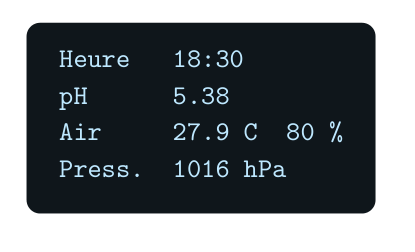
\includegraphics[width=0.3\textwidth]{img/inf/f_oled.png}
\caption{Contenu de l'écran avec le montage du 1\textsuperscript{er} novembre : heure 18:30, pH 5,38, air \qty{27,9}{\celsius} et \qty{80}{\percent}, pression \qty{1016}{hPa}.}
\end{figure}

% ---------------------------------------------------------------------
\Needspace{8\baselineskip}\subsection{Premières mesures réelles}

Une fois le matériel en service, j'enregistre les mesures pendant près d'une demi-heure, le 1er novembre de 18 h 20 à 18 h 48, avec les capteurs disponibles. Pendant cet essai, j'étalonne la sonde pH avec les solutions tampon pH 7 et pH 4, grâce aux boutons du dashboard. J'exporte les données depuis le dashboard (onglet Journal) et je les analyse ici. Cette sous-partie résume d'abord les mesures recueillies, puis compare le pH avant et après étalonnage. Elle montre ensuite ce que les valeurs du pH révèlent sur la précision de la mesure, et se termine par les anomalies repérées dans les données.

\subsubsection*{Les données recueillies}

143 mesures sont enregistrées, une toutes les \qty{11,6}{s} en moyenne (de \qty{11}{s} à \qty{14}{s}) : aux \qty{10}{s} d'attente prévues s'ajoute le temps de lecture des capteurs, surtout la sonde de l'eau, que le programme interroge même absente.

Le tableau suivant donne les mesures du 1\textsuperscript{er} novembre.

\begin{table}[H]
\centering
\small
\begin{tabularx}{\textwidth}{|l|l|c|c|c|c|}
\hline
\textbf{Grandeur} & \textbf{Capteur} & \textbf{Mesures} & \textbf{Minimum} & \textbf{Moyenne} & \textbf{Maximum} \\
\hline
pH (après étalonnage) & sonde pH sur A1 & 119 & 5,26 & 5,40 & 5,49 \\
\hline
Température de l'air & DHT20\ix{24} & 143 & \qty{27,8}{\celsius} & \qty{28,0}{\celsius} & \qty{28,1}{\celsius} \\
\hline
Humidité de l'air & DHT20\ix{24} & 143 & \qty{80}{\percent} & \qty{80}{\percent} & \qty{81}{\percent} \\
\hline
Pression de l'air & BMP280 & 143 & \qty{1016}{hPa} & \qty{1016}{hPa} & \qty{1016}{hPa} \\
\hline
\end{tabularx}
\caption{Mesures du 1er novembre.}
\end{table}

Pour le pH, la ligne du tableau ne garde que les mesures faites après l'étalonnage, hors un point isolé (voir la sous-partie suivante). L'air reste très stable pendant l'essai, ce qui est normal en intérieur sur une demi-heure : \qty{0,3}{\celsius} et \qty{1}{\percent} d'humidité d'écart. La pression, affichée au hPa près, ne bouge pas. EC, niveau, température de l'eau et batterie n'ont pas de valeur, leurs capteurs n'étant pas branchés ; la lumière, entre \qty{0}{\percent} et \qty{1}{\percent}, n'est que le bruit d'une entrée sans capteur.

\subsubsection*{Le pH avant et après étalonnage}

La courbe se lit en trois temps. Avant étalonnage (18 h 20 à 18 h 22), le programme utilise les valeurs par défaut du fabricant et affiche environ 4,5 : cette valeur n'a pas de sens physique tant que la sonde n'est pas étalonnée. Ensuite, dans la solution tampon pH 7 (18 h 24), la mesure monte à 6,88 -- 7,00 ; l'appui sur le bouton « pH 7,00 » enregistre la tension du moment comme référence. Enfin, après étalonnage (à partir de 18 h 25), le pH se stabilise à $5{,}40 \pm 0{,}04$ (moyenne $\pm$ écart-type, 119 mesures) dans l'eau mesurée.

La figure suivante montre le pH mesuré le 1\textsuperscript{er} novembre, avant et après étalonnage.

\begin{figure}[H]
\centering
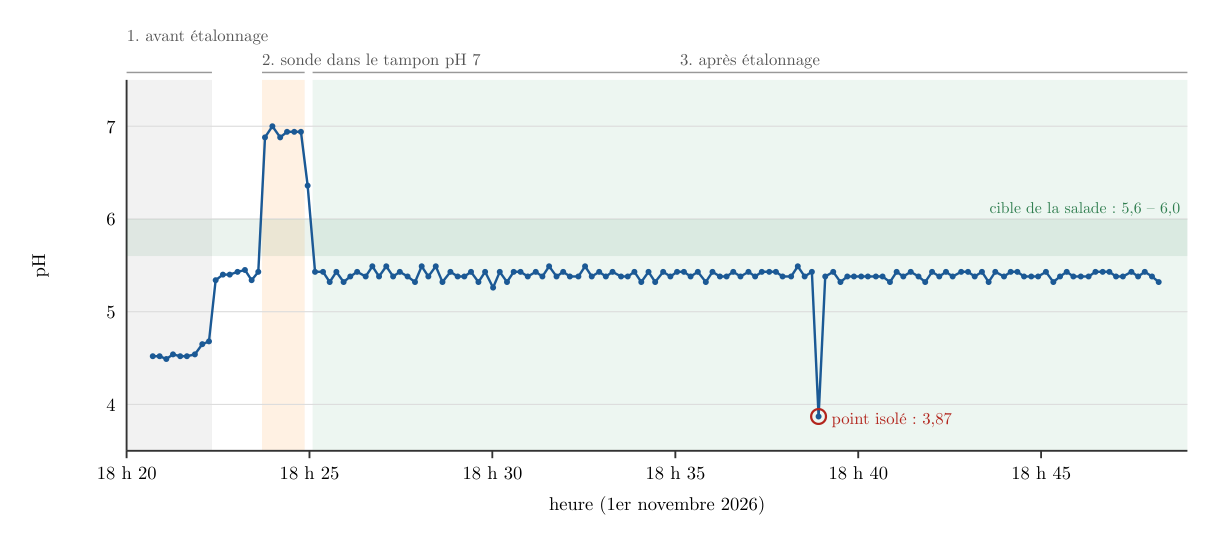
\includegraphics[width=\textwidth]{img/inf/f_ph_courbe.png}
\caption{pH mesuré le 1er novembre : avant étalonnage, dans la solution tampon pH 7, puis après étalonnage. La bande verte est la cible de la salade cultivée.}
\end{figure}

Cette valeur est en dessous de la cible de la salade (5,6 à 6,0). Le comportement attendu du pilote est alors de ne pas verser de pH$-$, qui ferait encore baisser le pH, et d'afficher l'avertissement « pH trop bas : pas de pH+, corriger à la main ». La mesure de 18 h 38 à 3,87 est un point isolé : la suivante revient aussitôt à 5,38. Elle correspond sans doute à une perturbation passagère (sonde bougée, bulle, faux contact). Une seule mesure de ce type ne déclenche pas de dose, puisque le pilote attend 10 minutes entre deux doses, mais un filtre qui écarte les valeurs isolées serait une amélioration utile.

\subsubsection*{La précision de la mesure du pH}

En regardant les valeurs une par une, je remarque que le pH ne prend que quelques valeurs bien précises : 5,26, 5,32, 5,38, 5,43 et 5,49. Ces « marches » sont la trace du convertisseur 10 bits de l'Arduino, qui ne distingue pas deux tensions séparées de moins de \qty{4,9}{mV}.

Le tableau suivant donne les valeurs de pH prises par la mesure après étalonnage.

\begin{table}[H]
\centering
\small
\begin{tabular}{|l|c|c|c|c|c|}
\hline
\textbf{pH affiché} & 5,26 & 5,32 & 5,38 & 5,43 & 5,49 \\
\hline
\textbf{Nombre de mesures} & 1 & 15 & 50 & 46 & 7 \\
\hline
\end{tabular}
\caption{Valeurs de pH prises par la mesure après étalonnage.}
\end{table}

\naturecalc{mesures du 1\textsuperscript{er} novembre sur le vrai matériel, comparées à la théorie}
\begin{demonstration}[ce que vaut une marche]
\resultat{\left|\Delta\mathrm{pH}\right| \approx 0{,}0275 \text{ par pas du convertisseur}}
D'après la droite d'étalonnage de la partie 8.4, le pH vaut $\mathrm{pH} = 7 + (U - U_7)\times\dfrac{4-7}{U_4 - U_7}$. Si la tension varie de $\Delta U$ (en mV), le pH varie de $\Delta\mathrm{pH}$ avec :
\begin{align*}
\mathrm{pH} + \Delta\mathrm{pH} &= 7 + (U + \Delta U - U_7)\times\frac{-3}{U_4 - U_7}\\
\Delta\mathrm{pH} &= \Delta U\times\frac{-3}{U_4 - U_7}
\end{align*}
En valeur absolue, la marche du pH vaut donc :
\[
\left|\Delta\mathrm{pH}\right| = \Delta U\times\frac{3}{U_4 - U_7}
\]
Une marche du convertisseur de l'Arduino correspond à un pas de $\Delta U = \dfrac{\qty{5000}{mV}}{1024} \approx \qty{4,88}{mV}$. L'étalonnage de la partie 8.4 donne $U_4 - U_7 = \qty{532}{mV}$, soit $\qty{532}{mV}/3 \approx \qty{177}{mV}$ par unité de pH. Pour un pas :
\begin{align*}
\left|\Delta\mathrm{pH}\right| &= \qty{4,88}{mV}\times\frac{3}{\qty{532}{mV}}\\
\left|\Delta\mathrm{pH}\right| &\approx 0{,}0275
\end{align*}
Les marches observées dans le relevé valent en moyenne, entre les valeurs extrêmes de 5,26 et de 5,49 séparées par 4 marches :
\begin{align*}
\Delta\mathrm{pH} &= \frac{5{,}49 - 5{,}26}{4}\\
\Delta\mathrm{pH} &= \frac{0{,}23}{4} = 0{,}0575
\end{align*}
Cela fait environ deux pas du convertisseur ($0{,}0575/0{,}0275 \approx 2{,}1$) : le bruit de la mesure saute souvent de deux pas à la fois. Avec l'ADS1115\ix{16} (pas de $\qty{0,1875}{mV}$ dans la plage par défaut), un pas ne vaudrait plus que :
\begin{align*}
\left|\Delta\mathrm{pH}\right| &= \qty{0,1875}{mV}\times\frac{3}{\qty{532}{mV}}\\
\left|\Delta\mathrm{pH}\right| &\approx 0{,}0011
\end{align*}
soit environ 26 fois moins que $0{,}0275$.
\end{demonstration}

Avec l'Arduino seul, le pH n'est donc connu qu'à environ \num{0,06} près (deux pas de bruit, soit \num{0,0575}). C'est suffisant pour surveiller, mais un peu juste pour doser au plus près d'une cible large de \num{0,4} seulement. Ces mesures confirment, avec des chiffres réels, le choix de l'ADS1115\ix{16} fait dans la partie 8.2.

\subsubsection*{Les anomalies des données}

L'export des journées du 31 octobre et du 1er novembre contient aussi des valeurs que j'écarte de l'analyse, parce qu'elles témoignent de défauts plutôt que de la réalité :

\begin{itemize}
\item \textbf{pH négatif le 31 octobre} (101 mesures, de $-5{,}91$ à $-0{,}20$) : enregistré avec l'ancien montage et sans étalonnage, il est physiquement impossible. Il montre qu'une mesure non étalonnée ou mal raccordée peut être totalement fausse, et pourquoi le pilote doit limiter le nombre de doses par jour.
\item \textbf{Température de l'eau à \qty{0,0}{\celsius}} le 1er novembre, sans aucune sonde branchée : c'est le deuxième défaut de la mise en service, corrigé depuis.
\item \textbf{Six lignes à l'heure incohérente} (de 19 h à 23 h le 1er novembre, alors que l'essai se déroule vers 18 h 30) : elles viennent probablement de la remise à l'heure au démarrage du serveur (horloge à pile ou Internet). Je les écarte ; ce point reste à vérifier.
\end{itemize}

\begin{aretenir}
Toute la chaîne de mesure fonctionne sur le vrai matériel : de la sonde au dashboard, en passant par l'Arduino, le Raspberry et la base de données. La sonde pH étalonnée donne une mesure stable ($\pm\num{0,04}$) ; sa finesse est limitée par le convertisseur de l'Arduino, ce que l'ADS1115\ix{16} corrigera.
\end{aretenir}

